\section{Chancen und Risiken von künstlicher Intelligenz} \label{Chancen und Risken von KI}
Die Möglichkeiten der Anwendung von künstlicher Intelligenz sind sehr vielfältig. Sie bergen sowohl Chancen als auch Risiken mit sich. 
Infolgedessen sollen verschiedene Anwendungsmöglichkeiten von KI - Systemen dargestellt werden und auf ihre Chancen und Risiken hin untersucht werden. 

\subsection{Chancen beim Einsatz von künstlicher Intelligenz}
\subsubsection{intelligente Assistenten}
Das Unternehmen IBM hat maßgeblich den Begriff \enquote{Cognitive Computing} geprägt. Der Begriff bezieht sich auf Systeme,
die skalierbar lernen und durch zielgerichtete Schlussfolgerungen mit Menschen interagieren können.
Diese Systeme können auf komplexe Fragestellungen mit Hypothesen, logischen Argumenten und Empfehlungen antworten~\footcite[\vglf][\pagef 23]{Scherk.2017}.
Der deutsche Digitalverband Bitkom zählt zu den Kernmerkmalen eines solchen Systems die \textbf{Adaptivität} sich an ein verändertes Umfeld anzupassen, sowie die 
\textbf{Interaktivität} mit Nutzern in Interaktion zu treten und dabei durch \textbf{Iterativität} Ziele und Probleme im Dialog zu präzisieren. Dabei ist es in der Lage
aus Informationen, aus vielen unterschiedlichen Quellen, die richtigen Schlüsse zu ziehen, die sog \textbf{Kontextualität}~\footcite[\vglf][\pagef 23]{Scherk.2017}.

Kognitive System ermöglichen für den Anwender eine \enquote{persönliche} Interaktion in natürlicher Sprache. Dabei ziehen die Systeme aus strukturierten und unstrukturierten
Daten, wie Text, Bild oder Sprache, Informationen, z.B. was einem Nutzer wichtig ist und gestalten durch das Hinzufügen von Details wie Stimmung und Umgangston eine natürliche 
Kommunikation. 
Explorative kognitive Systeme können dabei eigenständige Hypothen entwickeln, eine komplette Darstellung der wissenschaftlichen Literatur und gesellschaftlichen
Diskussion bereitstellen oder die Konsequenzen einer Absicht erörtern~\footcite[\vglf][\pagef 24]{Scherk.2017}.

Durch die Verwendung solcher intelligenter Systeme steigen die Kenntnisse und Kompetenzen der Benutzer, aufgrund des Umfangs und der deutlich schnelleren Verfügbarkeit
von Wissen und dadurch steigenden Lernmöglichkeiten. Das Beispiel der Verbreitung von medizinischem Wissen verdeutlicht dies. 1950 
dauert es schätzungsweise ungefähr 50 Jahre, um das Wissen weltweit zu verdoppeln. 1980 waren es nur noch sieben Jahre und 2015 nur noch drei Jahre.
Die Systeme können Unternehmen und Organisationen helfen, mit der stetigen Entwicklung mitzuhalten und Ihre Leistungen zu verbessern~\footcite[\vglf][\pagef 25]{Scherk.2017}.

Im Einzelhandels- und Dienstleistungsgewerbe ermöglichen intelligente Assistenten bessere Produkte und Dienstleistungen durch die Interaktion mit den Kunden 
und die daraus resultierenden Schlussfolgerungen über dessen Vorlieben und Kaufverhalten.
Als Beispiel dient hier \enquote{H\&M Home Stylist}, ein Chatbot von der Firma H\&M, welcher den Kunden bei der Einrichtung Ihres Zuhauses unterstützt. Der Chatbot 
fragt den Kunden nach seinen Vorlieben und basierend auf seinen Antworten sucht der Chatbot passende Produkte für ihn aus. Mit Einführung des \enquote{H\&M Home Stylist}
wurde die Kundenzufriedenheit gesteigert und der Umsatz des Unternehmens erhöht~\footcite[\vglf][\pagef 53]{Robot.2023}.

Ebenfalls werden durch die Interaktion mit intelligenten Systemen neue Daten generiert, die wiederum ausgewertet werden können und aufgrund neu gefundener Muster neue Handlungshypothesen
ermöglichen.

Der immer stetig wachsende Einsatz von intelligenten Assistenten wird zahlreiche Arbeitsprofile, insbesondere von Wissensarbeitern, verändern. Es wird sich eine Arbeitsteilung 
zwischen dem kognitiven System und Menschen entwickeln, indem sie kooperieren. Dadurch entsteht eine Kombination aus den jeweiligen Stärken der beiden Entitäten, z.B. indem
die kognitiven Systeme die menschliche Kreativität in Innovationsprozessen verstärken~\footcite[\vglf][\pagef 25]{Scherk.2017}.
Ein Beispiel einer solchen Kooperation ist eine Investmentfirma aus Hongkong. Diese hat einem kognitiven System den Status eines Vorstandsmitgliedes übertragen. Ohne die Zustimmung
des Systems werden keine Investitionen mehr abgesegnet~\footcite[\vglf][\pagef 25]{Scherk.2017}.

\subsubsection{Robotik}
Die bereits erwähnte Kooperation ist besonders in der Robotik zu erkennen. Allein in Deutschland kommen ca. 1.8 Industrieroboter in der Arbeitswelt zum Einsatz und erleichtern
den Arbeitsalltag vieler Menschen. Allerdings soll es im folgenden Kapitel um sog. soziale Roboter gehen. In Deutschland sind künstlichen Gehilfen noch eine Ausnahmeerscheinung,
während diese in den USA und Japan bereits Alltag ist. Dort sind Wachroboter zur Überwachung der Besucher in Einkaufszentren, Flughäfen oder Restaurants und autonome Pizzaboten im Versuchsstadium im Einsatz. Ebenfalls werden Roboter in 
Altenheimen zur Rehabilitation und Therapie eingesetzt. Die Spannweite reicht dabei von einer Terminerinnerung über Nachhilfe bis hin zum Einsatz als Polizeiassistenten.
Auch können Sie als Kinderspielzeug, Babysitter oder sogar als ein Ersatz für eine persönliche Beziehung eingesetzt werden~\footcite[\vglf][\pagef 107]{Heinrichs.2022}.
Es ist davon auszugehen, dass die Interaktion mit sozialen Robotern in Zukunft eine Selbstverständlichkeit erreicht, die den Umgang mit dem Smartphone gleichzusetzen ist.

Grund für diesen Erfolg ist vor allem die Tatsache, dass diese künstlichen Gehilfen manche Arbeiten gleichwertig oder besser verrichten als ihr menschliches Pendant, aber auch
Arbeiten verrichtet, die für Menschen unliebsam sind. 
Vielen Menschen profitieren auch vom Umgang mit Robotern, insbesondere bei Therapien von Menschen, die den Kontakt zu Menschen meiden z.B. Autisten. Als weiteres Beispiel für die Arbeitserleichterung durch künstliche Gehilfen lassen sich 
Pflegeroboter anführen, die die physischen Lasten des meist weiblichen Personals reduzieren~\footcite[\vglf][\pagef 108]{Heinrichs.2022}.

\subsubsection{Autonomes Fahren}
Autonomes Fahren verspricht vor allem die Sicherheit im Straßenverkehr zu erhöhen, indem die Anzahl der Verletzten und Verkehrstoten reduziert wird. Zum aktuellen Zeitpunkt
gibt es bereits unzählige Fahrassistenzsysteme, wie z.B. automatische Einparkassistenten, die vor allem den Fortschritten in der Sensorik und im \ac{ML} zu verdanken sind.
Unfälle können bspw. vermieden werden, indem Gefahrensituationen im Voraus erkannt werden, indem auf Grundlage der Projektion von Bewegungspfaden von Verkehrsteilnehmern die Risikolage
von Kollisionen analysiert werden.
Bereits jetzt können selbstfahrende Autos mehrere tausend Kilometer unfallfrei zurücklegen, ohne die Notwendigkeit eines menschlichen Eingreifens~\footcite[\vglf][\pagef 29]{Scherk.2017}.

Die \ac{KI} wird einen wesentlichen Beitrag bei der Optimierung von Verkehrsflüssen leisten. Im Personen- und Warenverkehr können Staus vermieden werden, indem Verkehrsströme aufeinander 
abgestimmt werden und so die Verkehrsinfrastruktur entlasten. Auch können freie Kapazitäten erkannt und ausgenutzt werden, indem die Grünphasen von Ampeln an das momentane
Verkehrsaufkommen angepasst werden~\footcite[\vglf][\pagef 178]{Wittpahl.2018}. Diese Verbesserungen wären ein großer Schritt in Richtung umweltfreundliche Mobilität, da zum einen 
die Emissionen verringert und zum anderen der Verkehrsfluss optimiert werden würde. Auch andere ressourcenschonende Lösungen, wie die intelligente Ladezyklen Steuerung in der Elektromobilität
führt zu einer Verlängerung der Lebensdauer, bei gleichzeitiger Erhöhung der Reichweite~\footcite[\vglf][\pagef 178]{Wittpahl.2018}.
Für neue Mobilitätsformen wie autonome Flugtaxis oder Logistik-Drohnen wird zukünftig der Einsatz von KI ebenfalls eine entscheidende Rolle spielen~\footcite[][\pagef 178]{Wittpahl.2018}.

\begin{figure}[H]
    \centering
    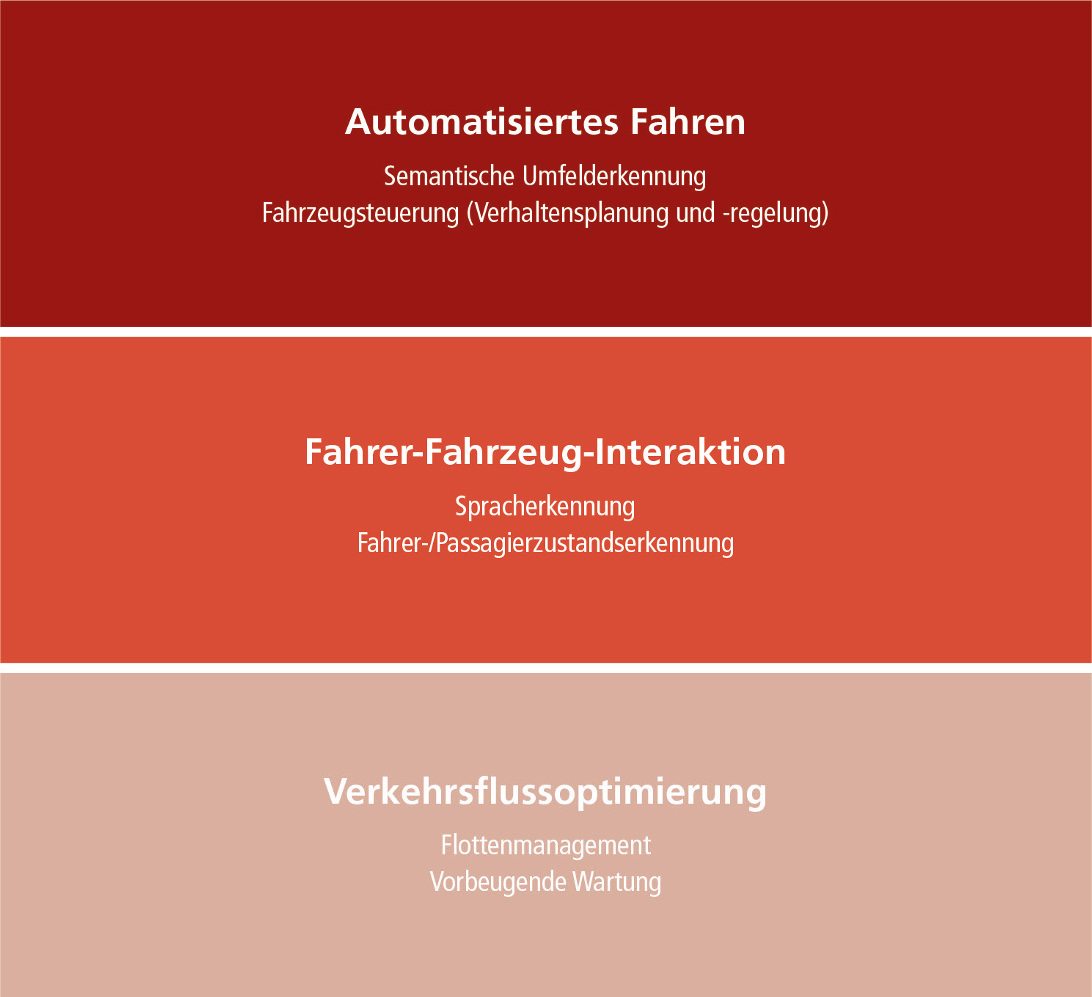
\includegraphics[width=0.8\textwidth]{AF} 
    \caption[Überblick der Anwendungsbereiche der KI für das automatisierte \mbox{Fahren}]{Überblick der Anwendungsbereiche der KI für das automatisierte \mbox{Fahren}\footnotemark}
    \label{fig:af}
\end{figure}
\footnotetext{\cite[\vglf][\pagef 179]{Wittpahl.2018}}

Wie in \autoref{fig:af} zu sehen ist, hat \ac{KI} neben dem automatisierten Fahren und der Verkehrsflussoptimierung auch noch die Aufgabe der Fahrer-Fahrerzeug-Interaktion. Der Mensch 
gibt immer mehr Verantwortung und Aufgaben an die \ac{KI} ab. Das hat den positiven Effekt, dass diese immer mehr Trainingsdaten erhält und sich dadurch stetig verbessert.
Hierdurch wird das Vertrauen in das autonome Fahren steigen und die Mobilität sich weiter wandeln~\footcite[\vglf][\pagef 188]{Wittpahl.2018}.

\subsubsection{Gesundheitsweisen}

Das Gesundheitsweisen profitiert besonders von der modernen Entwicklung in der \ac{KI}-Forschung. \ac{KI} kann in der medizinischen Forschung, bei der Diagnose sowie Behandlung 
von Krankheiten eingesetzt werden. Auch die Verwaltung von Gesundheitsdaten kann von der \ac{KI} übernommen werden~\footcite[\vglf][\pagef 177]{Robot.2023}.

Durch die sehr gute Musterkennung in großen Datensätzen können \ac{KI}-Systeme besonders vorteilhaft in der Medizin eingesetzt werden. Sie können die erkannten Muster mit
der Krankengeschichte des Patienten abgleichen und so Erkenntnisse hervorbringen, die ein menschlicher Arzt mit dem menschlichen Auge und der menschlichen kognitiven Limitierung nicht 
erkennen würde~\footcite[\vglf][\pagef 392]{Buchkremer.2020}. Sie sind auch in der Lage, bei der Diagnose und bei der Behandlung von Krankheiten zu helfen, 
da sie imstande sind, genetische Informationen eines Menschen zu analysieren oder seine medizinischen Bilder auszuwerten~\footcite[\vglf][\pagef 177]{Robot.2023}.

Es ist davon auszugehen, dass Ärzte in der näheren Zukunft nicht mehr allein agieren werden, sondern Sie ein Dreiergespann aus Arzt, Patient und Maschine bilden werden. 
Das hat den Vorteil, dass der Arzt bei seiner Diagnostik durch ein \ac{KI}-System unterstützt wird und so fehlerhafte Diagnosen verhindert werden können, denn ungefähr 
20-30\% aller Diagnosen im ambulanten Bereich sind zurzeit falsch~\footcite[\vglf][\pagef 392]{Buchkremer.2020}.

Aber auch das Gesundheitsweisen hat die Chance, einen positiven Einfluss auf die \ac{KI}-Entwicklung zu nehmen, indem eine gemeinsame Kooperation entsteht, in der offen kommuniziert wird.
Desto mehr die \ac{KI}-Entwicklung in den medizinischen Prozess eingebunden wird, umso mehr könnte das Gefühl entstehen, dem Gemeinwohl zu dienen und die eigenen
Interessen zurückzustellen. Dies würde einen positiven Effekt für alle Bereiche erwirken. Auch könnte der externe Einfluss auch eine Minimierung von 
Sicherheitsrisiken nach sich ziehen, da alle Teilnehmer altruistisch motiviert wären~\footcite[\vglf][\pagef 392]{Buchkremer.2020}. 
Wichtig wäre hierbei allerdings, dass das Ganze innerhalb der Grenzen des \ac{DSGVO} geschehen sollte, um die Sicherheit und die Persönlichkeitsrechte der Patienten zu wahren.

\subsection{Risiken beim Einsatz von künstlicher Intelligenz}
\subsubsection{Arbeitswelt}
Eine der größten Anwendungsbereiche von \ac{KI}-Systemen stellt der Wirtschaftssektor dar z.B. werden sie eingesetzt für die Rekrutierung von Personal und den Verkauf von Gütern zu optimieren oder um
Arbeitsprozesse in quantitativer und qualitativer Hinsicht zu verbessern. Der Einsatz von solche System ist auch mit der Hoffnung verknüpft, eine umfangreiche
Automatisierung aller Wirtschafts- und Arbeitsprozesse zu realisieren~\footcite[\vglf][\pagef 127]{Heinrichs.2022}.

Der Konsens vieler Autoren ist dabei gleich, dass es in der Zukunft viel weniger Bedarf für menschliche Arbeit gibt, besonders in Bereichen in dennen es viele
sich wiederholende und einfache Aufgaben gibt wie z.B. in der Produktion oder der Buchhaltung~\footcite[\vglf][\pagef 130]{Robot.2023}.
Das betrifft vorallem Bereich, in dennen niedrig qualifizierten Arbeitnehmern arbeiten. Besser qualifizerte Arbeitnehmen werden weiterhin 
benötigt, um die \ac{KI}-Systeme zu überwachen. Dies kann zu einer sozialen Ungleichheit führen, da Arbeitnehmer mit geringer Bildung 
und Qualifikation benachteiligt werden~\footcite[\vglf][\pagef 130]{Robot.2023}. Damit dieser Effekt gedämpft wird, müssen Arbeitnehmern
kontinuierlich geschult werden, um sie an den sich stetig verändernden Arbeitsmarkt anzupassen.
Dennoch werden Menschen, die keinen bis schlechten Zugang zu Bildung haben und nur wenig finazielle Ressourcen besitzen, ins Hintertreffen geraten. 
Unternehmen, Regierungen und Arbeitnehmern müssen sich auf die anstehenden Veränderungen einstellung und diesen Effekt durch eine besseren und leichtern
Zugang zu Bildung und Schulungen abfedern~\footcite[\vglf][\pagef 130]{Robot.2023}.

Je schneller die Automatisierung vorranschreitet, desto mehr Arbeitsplätze fallen weg. Der Einsatz von \ac{KI}-System schafft zwar auch neue hochqualifizerte 
Arbeitsplätze und senkt die Produktionskosten, aber die daraus entstehende Nachfrage durch automatisierten Prozess abgedeckt wirdd.
Innerhalb Amazons Lagerhalten arbeiten bereits mehr als 100.000 Roboter~\footcite[\vglf][\pagef 49]{Kipper.2020}.

Im Verlauf der Zeit wird die \ac{KI} in immer mehr Berufsfelder Einzug halten, auch in kogntive Berufe wie z.B. den Journalismus. Die Menschheit muss sich 
auf Lange sicht Wege und Möglichkeiten suchen, wie sie das gesellschaftliche Leben ohne Arbeit gestalten kann.
    
\subsubsection{Überwachung, soziale Kontrolle und Diskriminierung}

Big Data stellt ein großes Machtpotenzial dar, da durch die Datenherbung von Unternehmen und Regierungen unzählige Daten von Bürgern erfasst wurden. Die systematische 
Auswertung dieser Daten ermgölich es \ac{KI}-System dieses Machtpotenzial auszuschöpfen.
Als negatives Beispiel dient die Volksrepublik China. Unter dem Deckmantel eines Gesundheitsprogramms wurden in den Jahren 2016 bis 2017 biometrische Daten aller
Bewohner der Provinz Xinjiang gesammelt. Die Daten umfassen Blutgruppe, Irisscans, Stimmaufnahmen und DNA. Im Jahr 2019 wurde eine Datenbank mit den Daten von 2,5 Millionen
Einwohnern Xinjiangs entdeckt, die aufgrund der vorangegangen Datensammlung, mit modernster Überwachungstechnologie überwacht wurden~\footcite[\vglf][\pagef 33]{Kipper.2020}.
Weiter hat China 2020 ein Sozialkreditsystem eingeführt, welches ohne Gesichterkennung, Spracherekknung und der massenhaften Erfassung und Verarbeitung von Daten durch
\ac{KI}-Systeme nicht möglich wäre. Dieses System belohnt vermeindlich \enquote{gute} Bürger mehr Privilegien. Wohingehen \enquote{unsoziales Verhalten} zu einer Verringerung der
Sozialpunkte des Bürger führt. Dies hat für Ihn negative Auswirkungen, die von längeren Wartezeiten bei Behörden, bis hin zu Ablehnung bei Ticketkäufen für den öffentlichen Verkehr
reichen können. Der Fortschritt in der \ac{KI}-Forschung wird immer mehr Möglichkeiten eröffnen, Menschen zu kontrollieren~\footcite[\vglf][\pagef 33]{Kipper.2020}.

Auch in der westlichen Welt, wird die Auswertung von Daten durch \ac{KI}-Systeme verwendet, um Menschen zu kontrollieren, vornehmlich allerdings im privaten Sektor durch Werbung.
Über die Suchen bei Online-Suchmaschinen, aufrufen von Webseiten, oder Gesprächen in Reichweise eines digital Assisten wie z.B. Amazons \enquote{Alexa} wird den Bürgern
gezielt Werbung angezeigt. Künstliche neuronale Netze finden dafür bestimmte Attribute in Korrelation~\footcite[\vglf][\pagef 33]{Kipper.2020}.
Aus den resultierenden Daten kann auch abgeleitet werden, welche Schwächen ein Mensch besitzt, z.B. Online-Glückspiel. Die Gefahr, dass durch die wiederholte Anzeige von 
Glückspielwerbug, aufgrund eines einmaligen Suchvorgangs, ein Suchtverhalten ausgelöst wird, ist nicht unwahrscheinlich.
Aber es können auch Aussagen über das Kaufverhalten und der Zahlungsbereitschaf von Kunden getroffen werden. So finden sich in persönlicher Werbung oftmals deutlich
teurere Preise als allgemeiner Werbung.
Wenn Unternehmen auf der Basis immer größerer Datenmengen und immer besserer KI Konsumentenverhalten immer präziser vorhersagen und damit steuern können, 
könnte das zu einem gewaltigen Machtgefälle zu Ungunsten der Verbraucher führen~\footcite[\vglf][\pagef 35]{Kipper.2020}.


\subsubsection{Autonome Waffensysteme}

Bereits seit die ersten Schritte in der \ac{KI}-Forschung getan waren, war diese eng mit dem Militär verbunden. Der Militär-Apparat verwendet bereits Software, die Luftbilder auswerten kann,
über Exoskelette, die Soldaten mehr Kraft verleihen, bis hin zu Drohnen und zu System zur Kontrolle von Waffensystem, aus der \ac{KI} und Robotik.
In der Neuzeit kamen auch \enquote{Cyberschlachtfelder} hinu, wo um die Kontrolle von zivielen und militärischen Computersystem gekämpft wird~\footcite[\vglf][\pagef 86]{Lenzen.2020}.

Nach einem Bericht des Futere of Life Institute existieren momentan Weltweit 284 Waffensystem die autonom agieren können. Größtenteils handelt es sich dabei um Raketen,
die eine eigenständige Ziielsuche besitzen. Die Vorfilterung von Informationen und das eigenständige treffen von Entscheideung stellt dabei einen strategischen Vorteil dar. 

Der Mensch bekommt nur noch vorgefilterte Information durch ein Computersystem, was aufgrund der schieren Menge an Daten nicht anders möglich st. Letzendlich trifft dieser
die Entscheidung, allerdings stellen Froscher sich die Frage, inwieit ein Mensch aufgrund der vorgefilterten Informationen durch ein \ac{KI}-System wirklich relevant entscheiden~\footcite[\vglf][\pagef 88]{Lenzen.2020}.
zieht man alles in Betracht, so sind Szenarien vorstellbar, in dennen \ac{KI} gesteuerte Schwärme von Drohnen per Gesichtserkennung gezielt nach Personen suchen und diese liqudieren~\footcite[\vglf][\pagef 28]{Kipper.2020}.
Ebenfalls entsteht eine Verantwortungslücke, da eine \ac{KI} in keinster Weise zur Rechenschaft gezogen werden kann, und der menschlichte Akteur seine Verantwortung auf die 
\ac{KI} überträgt~\footcite[\vglf][\pagef 153]{Heinrichs.2022}.
Ihr können zwar die Regel des Völkerrechts einprogrammiert werden, dennoch empfindet sie keine Empathie oder besitzt Emotionen.
Autonome Waffensystem können auch die Hemmschwelle der beteiligten Parteien zur Konflikteskalation senken, da der Einsatz von autonomen Waffensystemen nicht den Einsatz 
von menschlichen Soldate, auf dem Schlachtfeld, benötigt.
Aufgrund der übermenschlichen Geschwindigkeit der Datenverarbeitung von solchen System, könnte eine solche Situation eskalieren und nicht mehr kontrollierbar durch den Menschen werden.
Eine fatale Situation bei der enormen Zerstörungskraft solcher Systeme.

Ein Vorteil ist nicht von der Hand zu weisen, durch den Einsatz von autonomen Waffensystem, wird die Anzahl der menschlichen Beteiligten an einem Kampfgeschehen minimiert und 
somit auch die Opferzahlen~\footcite[\vglf][\pagef 30]{Kipper.2020}.